\chapter{Energy Calibration of the AHCAL}
\label{chap:ECalibAHCAL}

The CALICE Analog Hadronic Calorimeter (AHCAL) technological prototype was installed at the SPS CERN facilities in July and August 2015, in order to provide energy and time measurements of electromagnetic and hadronic showers using plastic scintillators. The data recorded in each cells of the calorimeter is measured in ADC counts, thus this scale cannot be compared directly between different channels. Therefore to compare them, all channels have to be scaled to a common physical energy unit. For the AHCAL, the Minimum Ionizing Particle or MIP unit is chosen. This unit relates to the cell energy in a well and understood physical process almost independent to outside conditions.

The conversion requires a calibration of each cells of the calorimeter which is by itself a challenge due to the high number of readout channels. In this testbeam, 3744 channels have to be calibrated. Due to the boards equipped with SiPMs from various different batches, the procedure needs to be automatic and robust to extract the calibration constant for each channel. At the end, all the calibration constants are entered in the official CALICE database.

This chapter will firstly describe the beamline facilities used in July 2015 at CERN, followed by the description of the tesbeam setup and finally describe the procedure performed for the AHCAL energy calibration.

\section{Beamline Setup}
\label{sec:beamline}

During the summer of 2015, CALICE performed several testbeam campaigns with the AHCAL technological prototype. The detector was installed in the beamline H2 at the North Area beamline at CERN \cite{H2Beamline}. The beamline provided wire chambers and scintillators that enabled us to have informations about the beam position and number of particles but unfortunately no data from theses detectors were recorded. Few information was collected about the amount of material upstream of the detector until the last momentum selection magnet. A Cherenkov detector (at around 500 m upstream) was also available to tag incoming particles. These detectors make advantage of the fact, a particle that traverses a medium faster than the speed of light in that medium will generate a cone of Cherenkov light \cite{}. This light can then be collected by a photomultiplier. The detector at this beamline offered the possibility to set a threshold for particle tagging. Usually, the threshold is set to distinguish between electrons and pions/kaons. This is particularly needed to tag electrons in pion runs. The tagging signal provided by the Cherenkov detector was fed to several AHCAL channels in order to be able to tag events.\\

For the production of particles, a primary high intensity proton beam (around $10^{12}$ protons per burst) of 400 GeV is impinged on a target. From this a secondary beam is produced containing various particles type and energies. For muons, the beam is obtained by scrapping the halo of a pion beam with collimators. For electrons, a neutral beam of photons is send to a lead target to generate electrons from gamma conversion, producing a very pure electron beam. For pions, the beam is selected via a set of collimators and magnets. Due to the decay of $\pi_0$ and the acceptance of the beamline, a contamination of the pion beam with electrons is possible at low momentum (< 20 GeV).

\section{Testbeam Setup}
\label{sec:TBsetup}

In July 2015, the AHCAL detector was using the full EUDET steel stack \cite{EUDET-Report-2010-02} with 48 iron absorber plates. Of it, 14 layers of active material was available for this testbeam as shown in figures \ref{fig:Det_layout} and \ref{fig:AHCAL_photo}. The data was recorded with beam from 10 to 90 GeV. The detector was placed on a movable stage, in order to be able to move the detector relative to the beam for muon calibration runs. This thesis will analyze muon data, electron showers between 10 and 50 GeV and pion showers between 10 and 90 GeV focusing on the timing aspect of the detector.

\begin{figure}[htbp!]
	\centering
	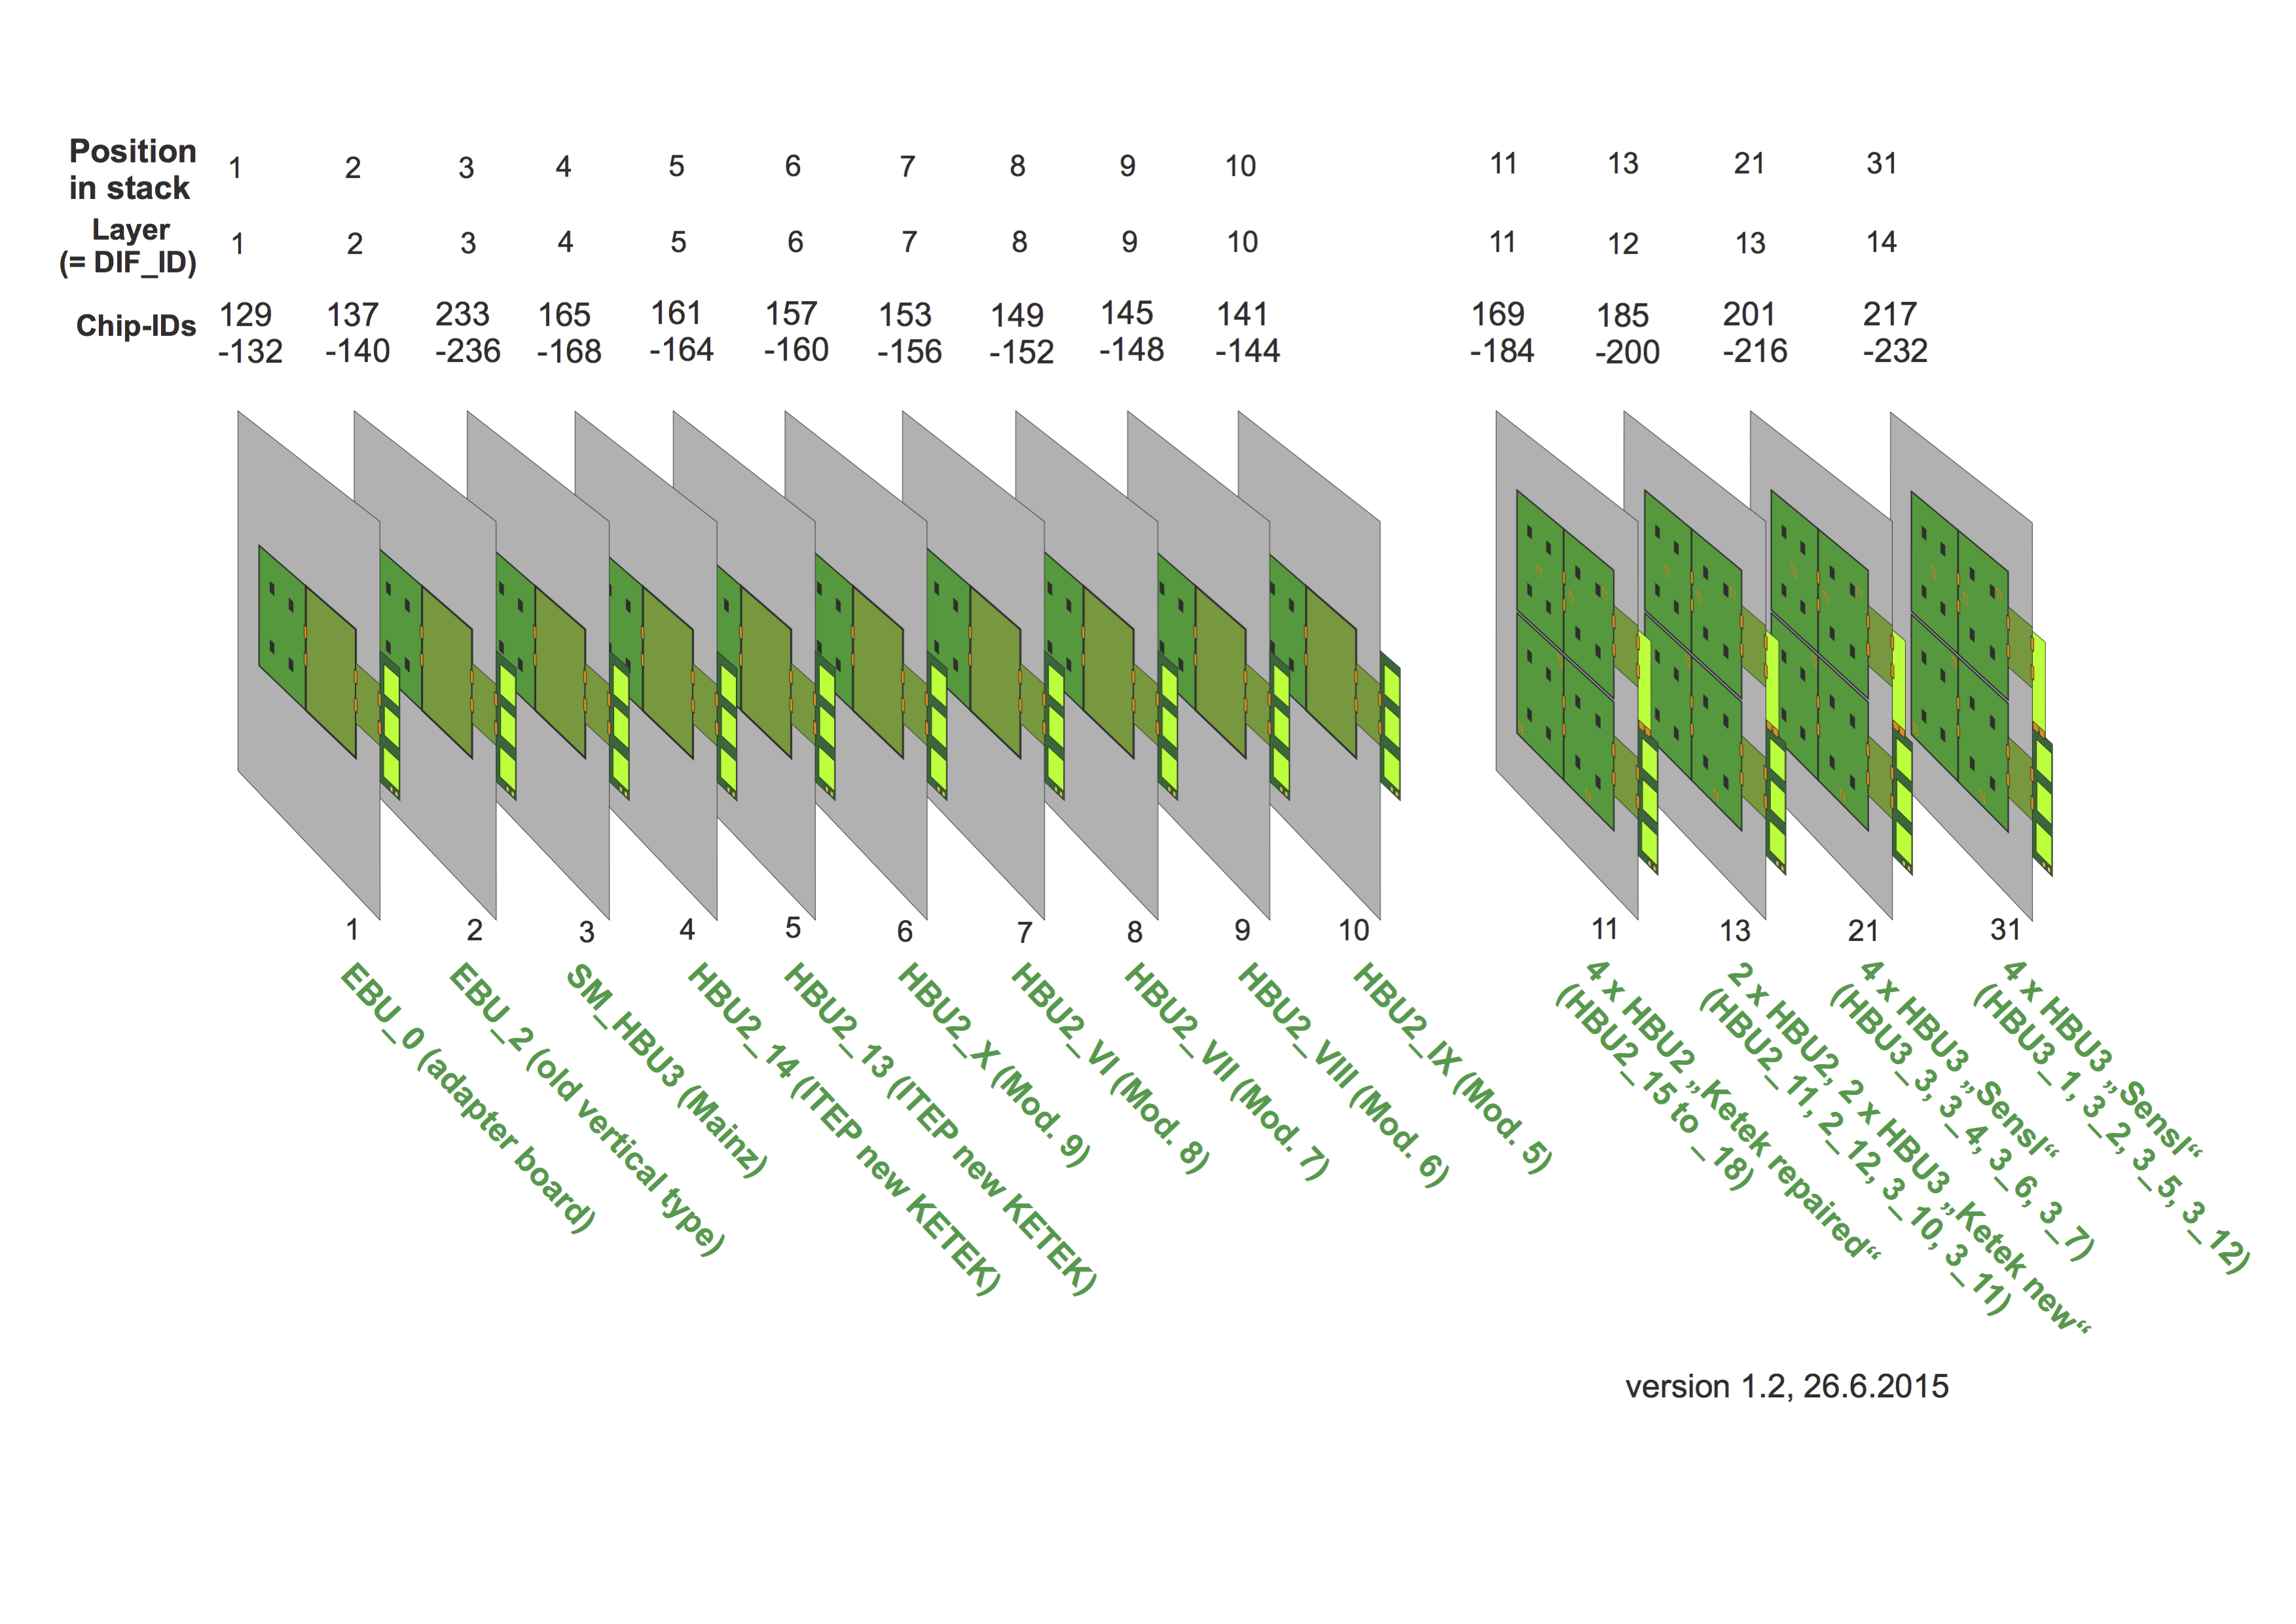
\includegraphics[width=1\linewidth]{chap5/fig_EnergyCalib/Detector_layout.png}
	\caption{Simplified view of the detector layout.} \label{fig:Det_layout}
\end{figure}

The beam instrumentation was consisted of two $10 \times 10$ cm$^2$ (in front of the calorimeter) as well as two $50 \times 50$ cm$^2$ (in front and back) scintillator plates readout with photomultiplier tubes. The coincidence of the $50 \times 50$ cm$^2$ scintillator was used for the muon runs and the coincidence of the $10 \times 10$ cm$^2$ scintillator was used for the electron and pion runs. Additionally, the coincidence signal from the scintillator was fed to several channels in the AHCAL in order to provide a reference time for the trigger which is important in this analysis.

\begin{figure}[htbp!]
	\centering
	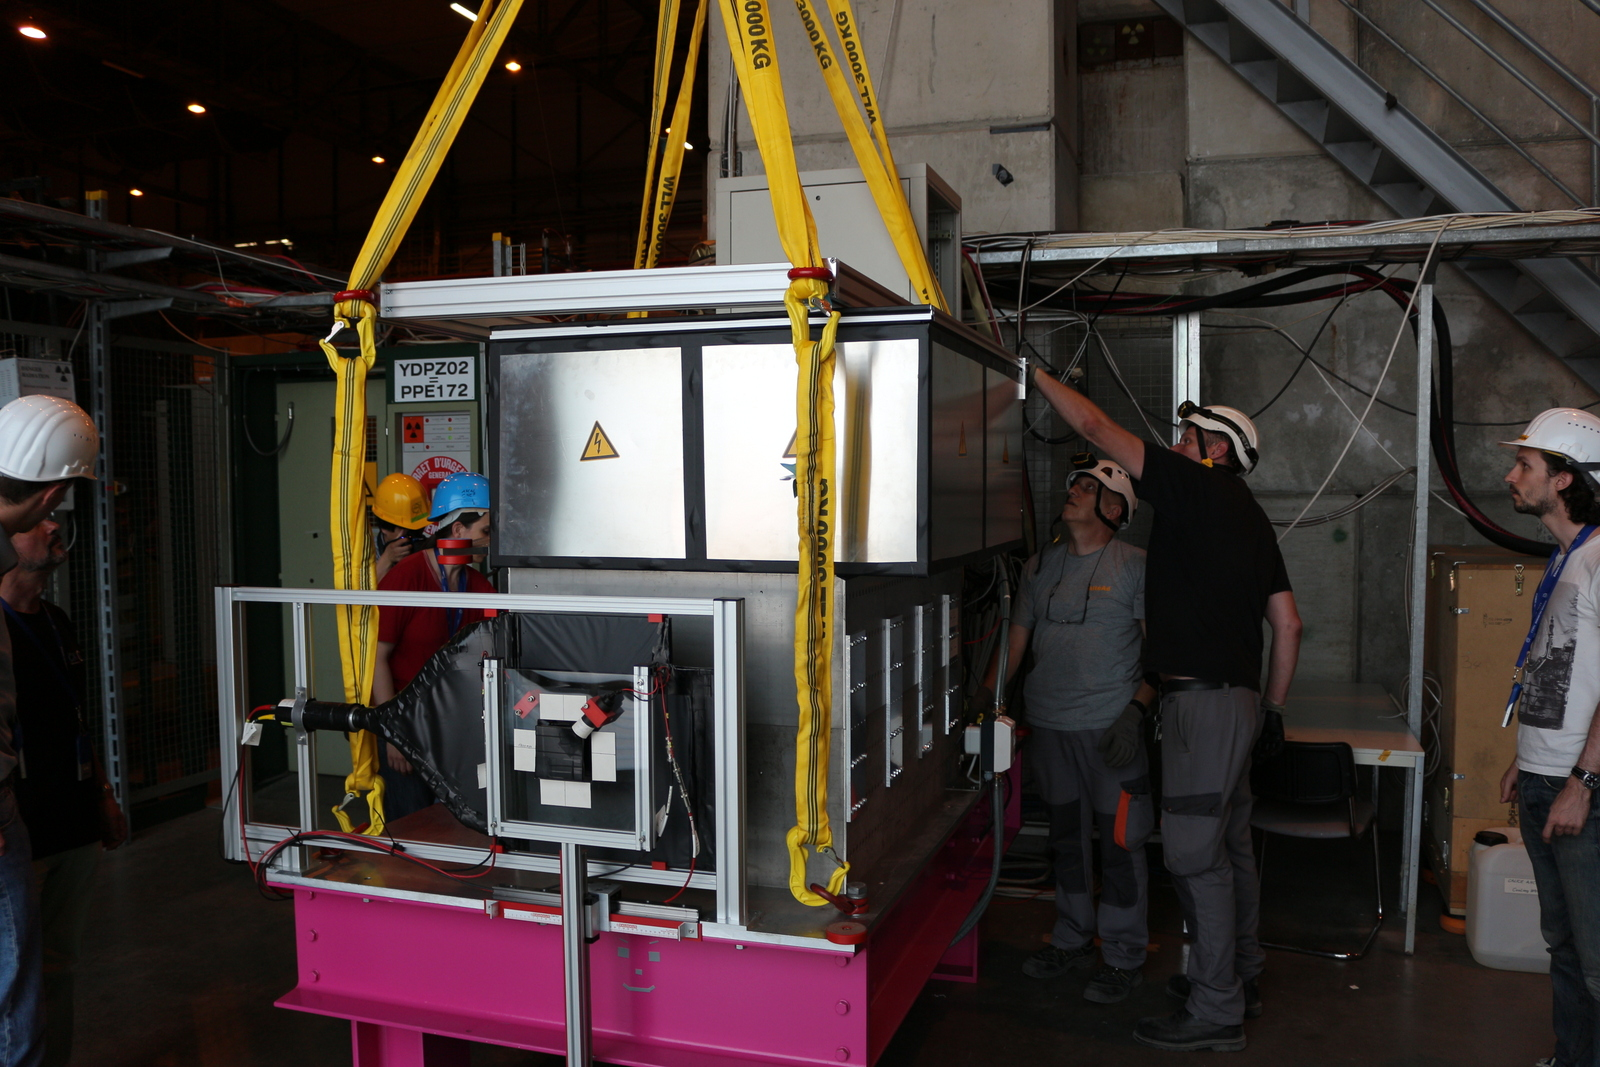
\includegraphics[width=0.7\linewidth]{chap5/fig_EnergyCalib/IMG_1170.jpg}
	\caption{Photo of the AHCAL detector before the installation in the testbeam area.} \label{fig:AHCAL_photo}
\end{figure}

\section{Testbeam monitoring}

It is important to monitor the data acquired during Testbeam. During testbeam, this is done at two level. On a pure hardware level, this is ideal to check fast that all layers are working as intended based on basic data. On a reconstructed level, this reflect more the data quality based on physics observables. For the former, a tool was already made and developed by the AHCAL group to check basic ADC/TDC, trigger informations channel-wise. Recently a shift has been done to a new monitoring tool developed in the AIDA2020 framework called DQM4HEP \cite{}. For the latter, no tool was available for shifters without the knowledge of the framework. This is why I developed a tool based on Qt and the ILCSoft framework called \textit{QtReco}. The tool is available on Github \cite{GithubTB}.

Simply, this tool is user-friendly by its interface and enables shifters to check physics observables as shower profiles, center of gravity, total energy with the acquired data in a quasi-online way. The tool is using the Marlin framework and the CALICE software package in order to reconstruct the data. A simple analysis module produce the necessary plots that are stored into a rootfile. A client can be used in order to get the desired plots based on server-socket communication. An example of the monitoring software can be seen in figures \ref{fig:QtReco_Server} and \ref{fig:QtReco_Client}.

\begin{figure}[htbp!]
	\begin{subfigure}[t]{0.5\textwidth}
		\centering
		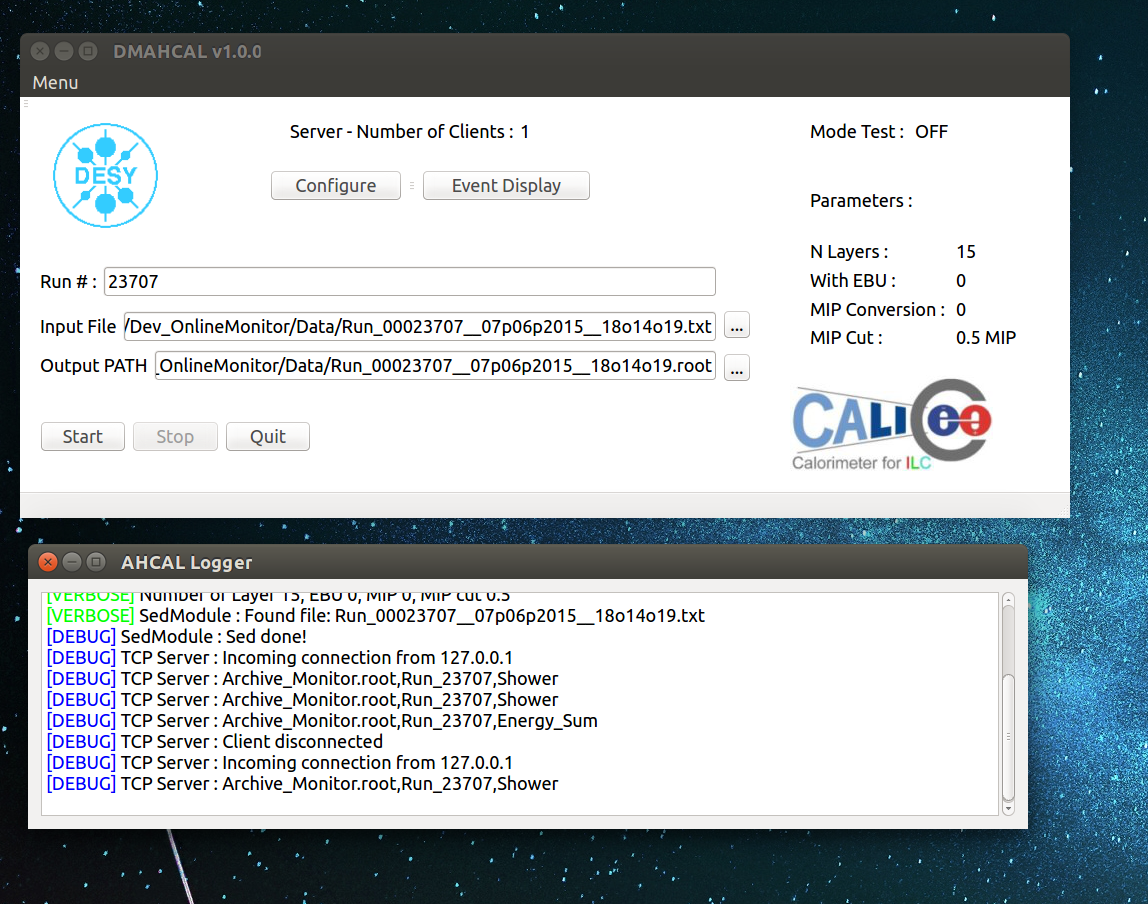
\includegraphics[width=1\linewidth]{chap5/fig_EnergyCalib/QtReco_Marlin.png}
		\caption{} \label{fig:QtReco_Server}
	\end{subfigure}
	\hfill
	\begin{subfigure}[t]{0.5\textwidth}
		\centering
		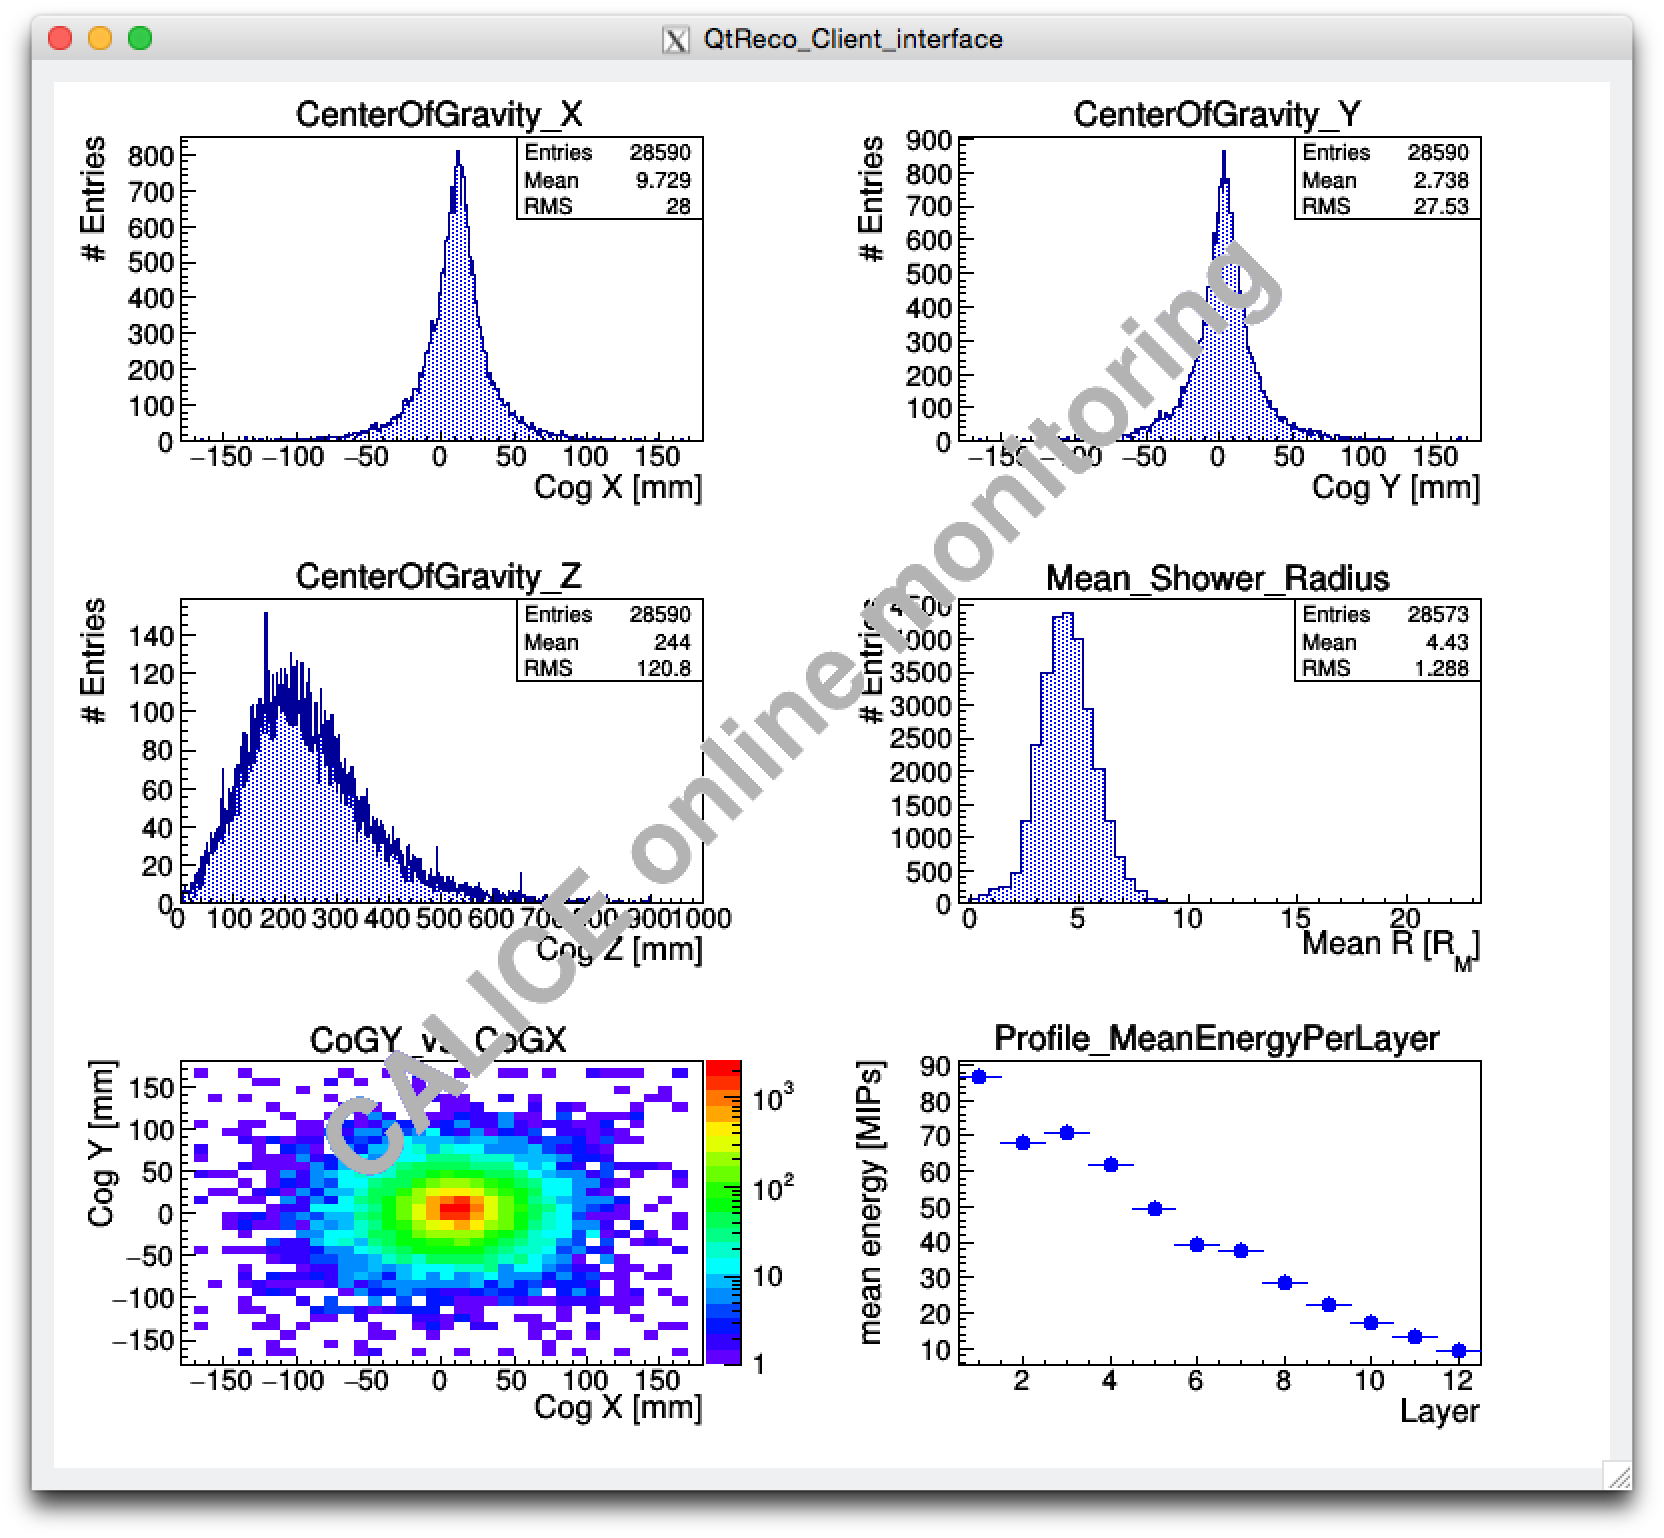
\includegraphics[width=1\linewidth]{chap5/fig_EnergyCalib/Shower_pion.png}
		\caption{} \label{fig:QtReco_Client}
	\end{subfigure}
	\caption{\subref{fig:QtReco_Server}) The server-side of the monitoring software. It is used to enter the parameters of the run via a steering file and reconstruct the data acquired quasi-online. \subref{fig:QtReco_Client}) Example of the plots obtained with the software from the client-side.}
\end{figure}

\section{Energy Calibration of the AHCAL}

Every channel of the detector provides a measure of the energy deposited in ADC units. To compare them or combined them, all channels need to be normalized to a common physics scale. The AHCAL uses muons to provide the calibration to the common scale as Minimum Ionizing Particles or MIP. Therefore muon runs were recorded. As detailed in section \ref{}, the energy deposited in a single AHCAL cell follows approximatively a Landau distribution but due to the electronic noise, the resulting response is convoluted with a Gaussian distribution. The maximum of the Laudau-Gaussian convolution density function is defined as the MIP constant ($M_{i}$) for the i-th channel. The full calibration is expressed as:

\begin{equation}
	E_i [MIP] = \frac{(A_i [ADC] - Ped_i [ADC]) \times IC_i }{ICP_i \times M_{i} [\frac{ADC}{MIP}]}
\end{equation}

where $E_i$ is the calibrated amplitude in MIP, $A_i$ the measured amplitude in ADC, $Ped_i$ the pedestal in ADC, $ICP_i$ the intercalibration between calibration and physics mode, $IC_i$ the intercalibration between High/Low gain and $M_{i}$ the MIP constant of the i-th channel. This formula is used in the case of no correction is performed for the SiPM saturation.

\subsection{Pedestal extraction}

To obtain the correct MIP constant, a pedestal subtraction has to be done. The pedestal value for each channels is extracted from the data taking muon runs. In order to be consistent, the pedestal value is extracted in the same running mode as data taking .i.e in auto-trigger (AT). For each channel and memory cell, an histogram is filled with the ADC value of a cycle in case no Hit Bit is set for the channel. The extraction is performed in an iterative way due to a high tail in energy that is not yet understood.

\begin{figure}[htbp!]
	\centering
	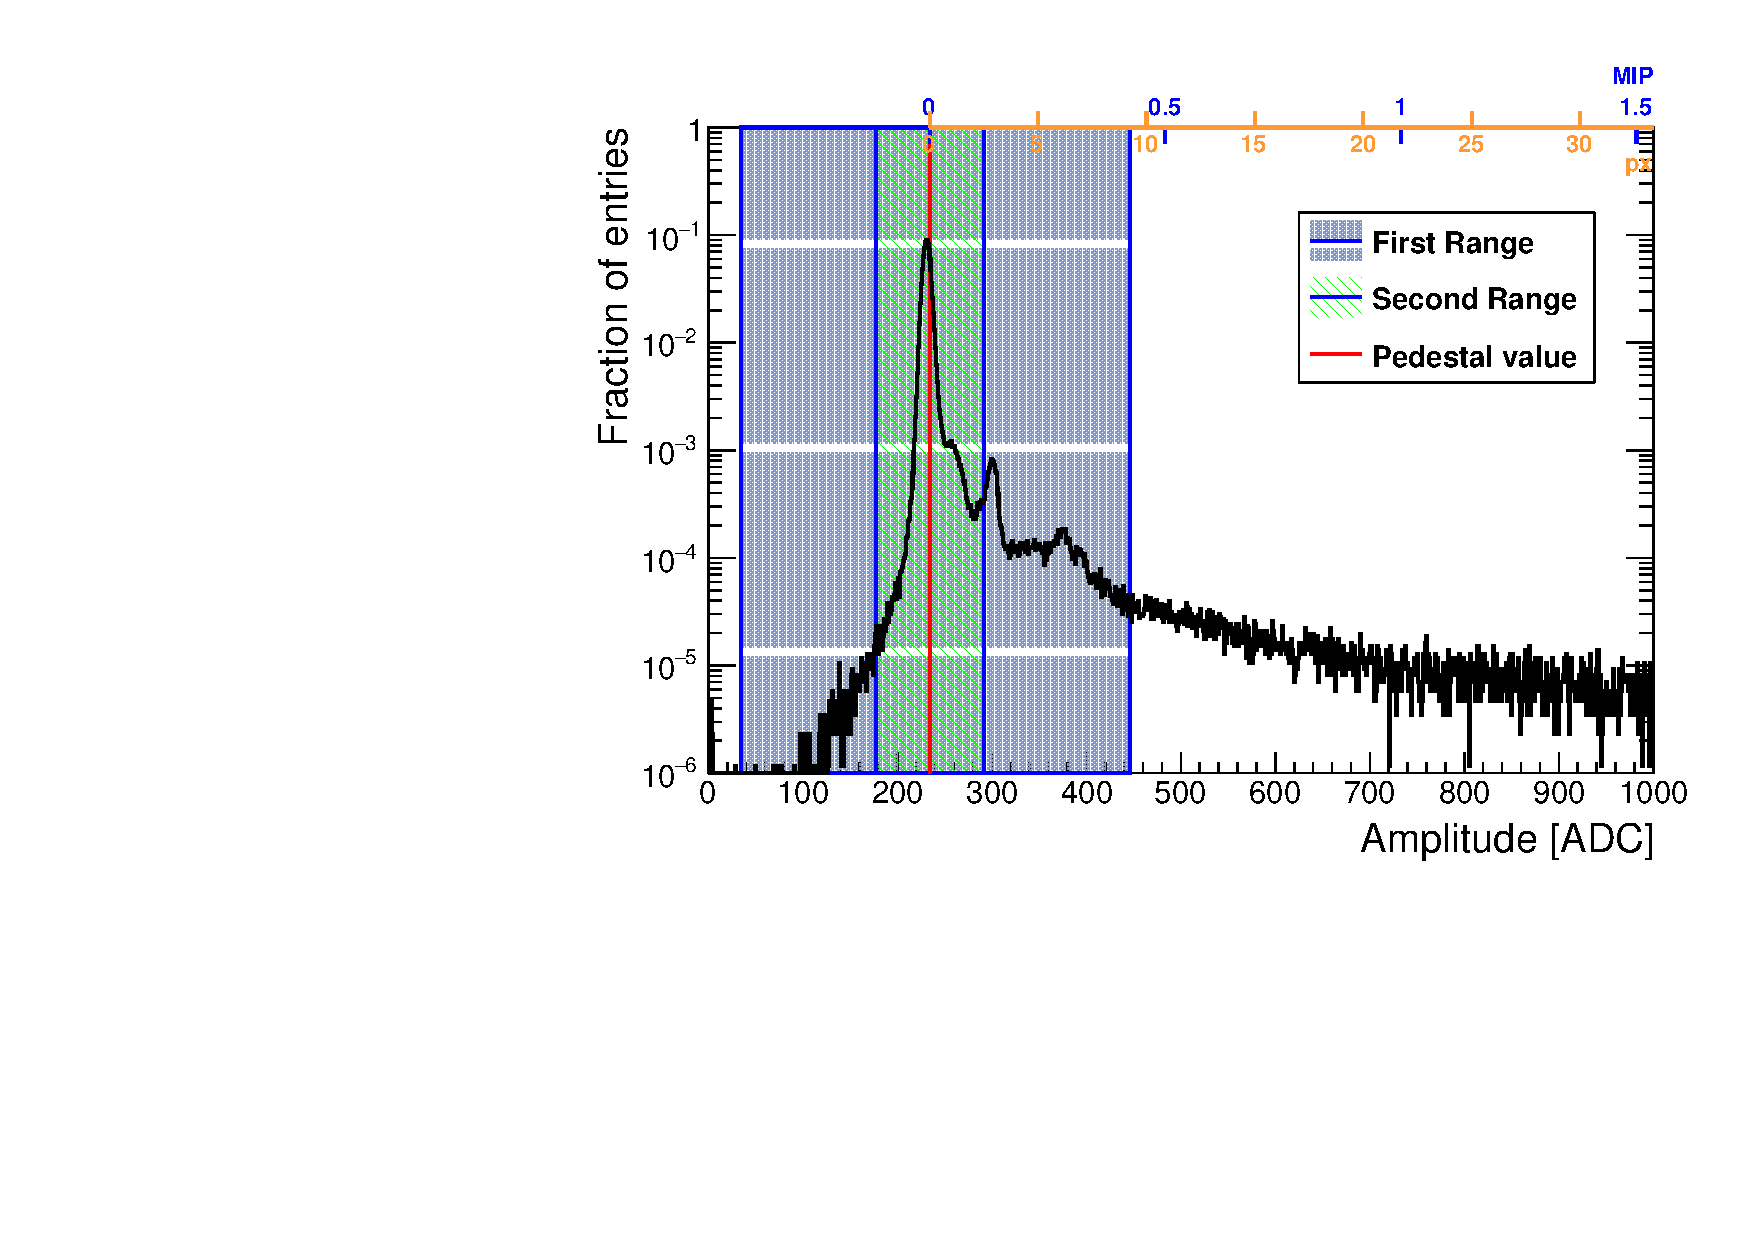
\includegraphics[width=0.7\linewidth]{../Thesis_Plots/EnergyCalib/Plots/PedestalExtractionExample.pdf}
	\caption{Typical pedestal distribution of a channel in auto-trigger mode. The different colored boxed represent the iterative procedure to extract the pedestal value marked with the red line.} \label{fig:PedExtraction}
\end{figure}

As the SiPM noise needs to be taken into account for the pedestal value and considering a poisson statistic, one to three pixels could be fired due to DCR and cross-talk. The fitting range then needs to be in the same order of magnitude of 1 to 3 pixels. For this, the histogram is reduced in the range of 3 RMS around the mean 2 times. After the mean of the histogram is taken the pedestal value as shown in figure \ref{fig:PedExtraction}. As no pedestal subtraction memory cell-wise is performed in the reconstruction at the moment and the database structure is not designed to have the pedestal constant for each memory cell, a mean over all memory cell is computed per channel. The average difference between the mean pedestal and the memory cell wise pedestal shown in figure \ref{fig:CompMeanMem} is around 21 ADC which would correspond to an error of about 4\% on the MIP constant (assuming a MIP value of 500 ADC). This error is dominating in the MIP constant uncertainty.

\begin{figure}[htbp!]
	\centering
	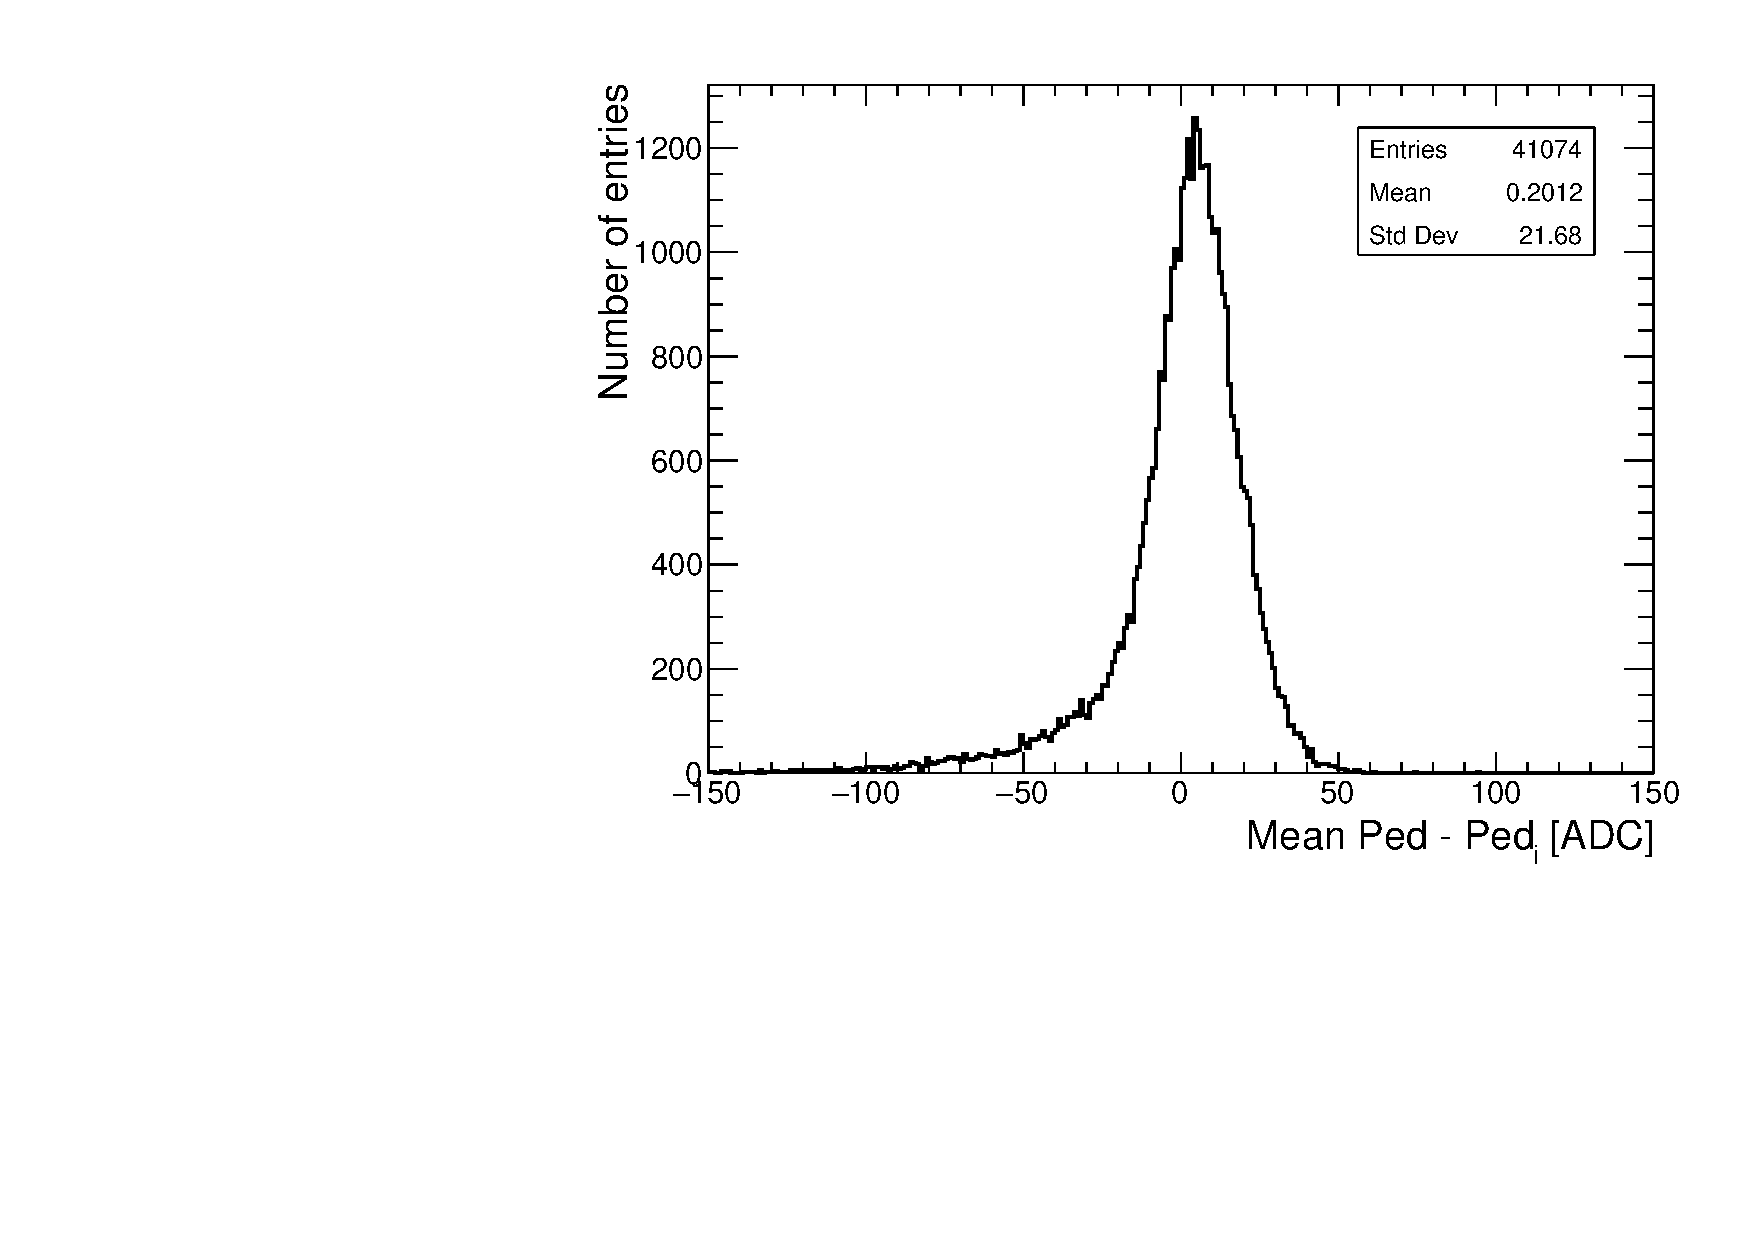
\includegraphics[width=0.7\linewidth]{../Thesis_Plots/EnergyCalib/Plots/ComparisonMeanPedtoMemorycell.pdf}
	\caption{Distribution of the difference between the mean pedestal to the memory-cell wise pedestal per channel.} \label{fig:CompMeanMem}
\end{figure}

\subsection{MIP extraction}

After the pedestal calibration, the extraction of the MIP constant for each channel can be performed. As the detector was equipped with various types of SiPM and boards designs, the extraction procedure needed to be automatized and robust. In order to reduce noise in the energy spectra of each cell that would lead to unstable fits and wrong MIP constants, a simple tracking selection has been performed as explained in section \ref{subsec:Muon_sel}.

After the selection, an histogram for each channel is filled with the energy value of each hit in ADC which are already pedestal subtracted. Then the fitting procedure is performed. The fitting procedure is very sensible to the initial parameters of the fit and can be quite difficult with the variety of SiPM and tiles in the AHCAL. To ensure a good fit, an iterative fitting procedure is performed. Only channels with more than 1000 entries are considered. First, the area is fitted. Secondly, the other parameters are released and fitted as well. Finally a final fit is performed on the four parameter in the range in the range of 30\% of the maximum of the previous fitted function. The detailed procedure is explained in \cite{FabianThesis}. A typical example of a MIP fit can be seen in figure \ref{fig:MIPFit}. Moreover, in order to fit possible channel that failed on the first attempt, an iteration of the procedure is done again on histograms that are filled with the energy of the hit for hits above 0.5 times the MPV value of the channel, if no value was fitted and estimation is used.

\begin{figure}[htbp!]
	\centering
	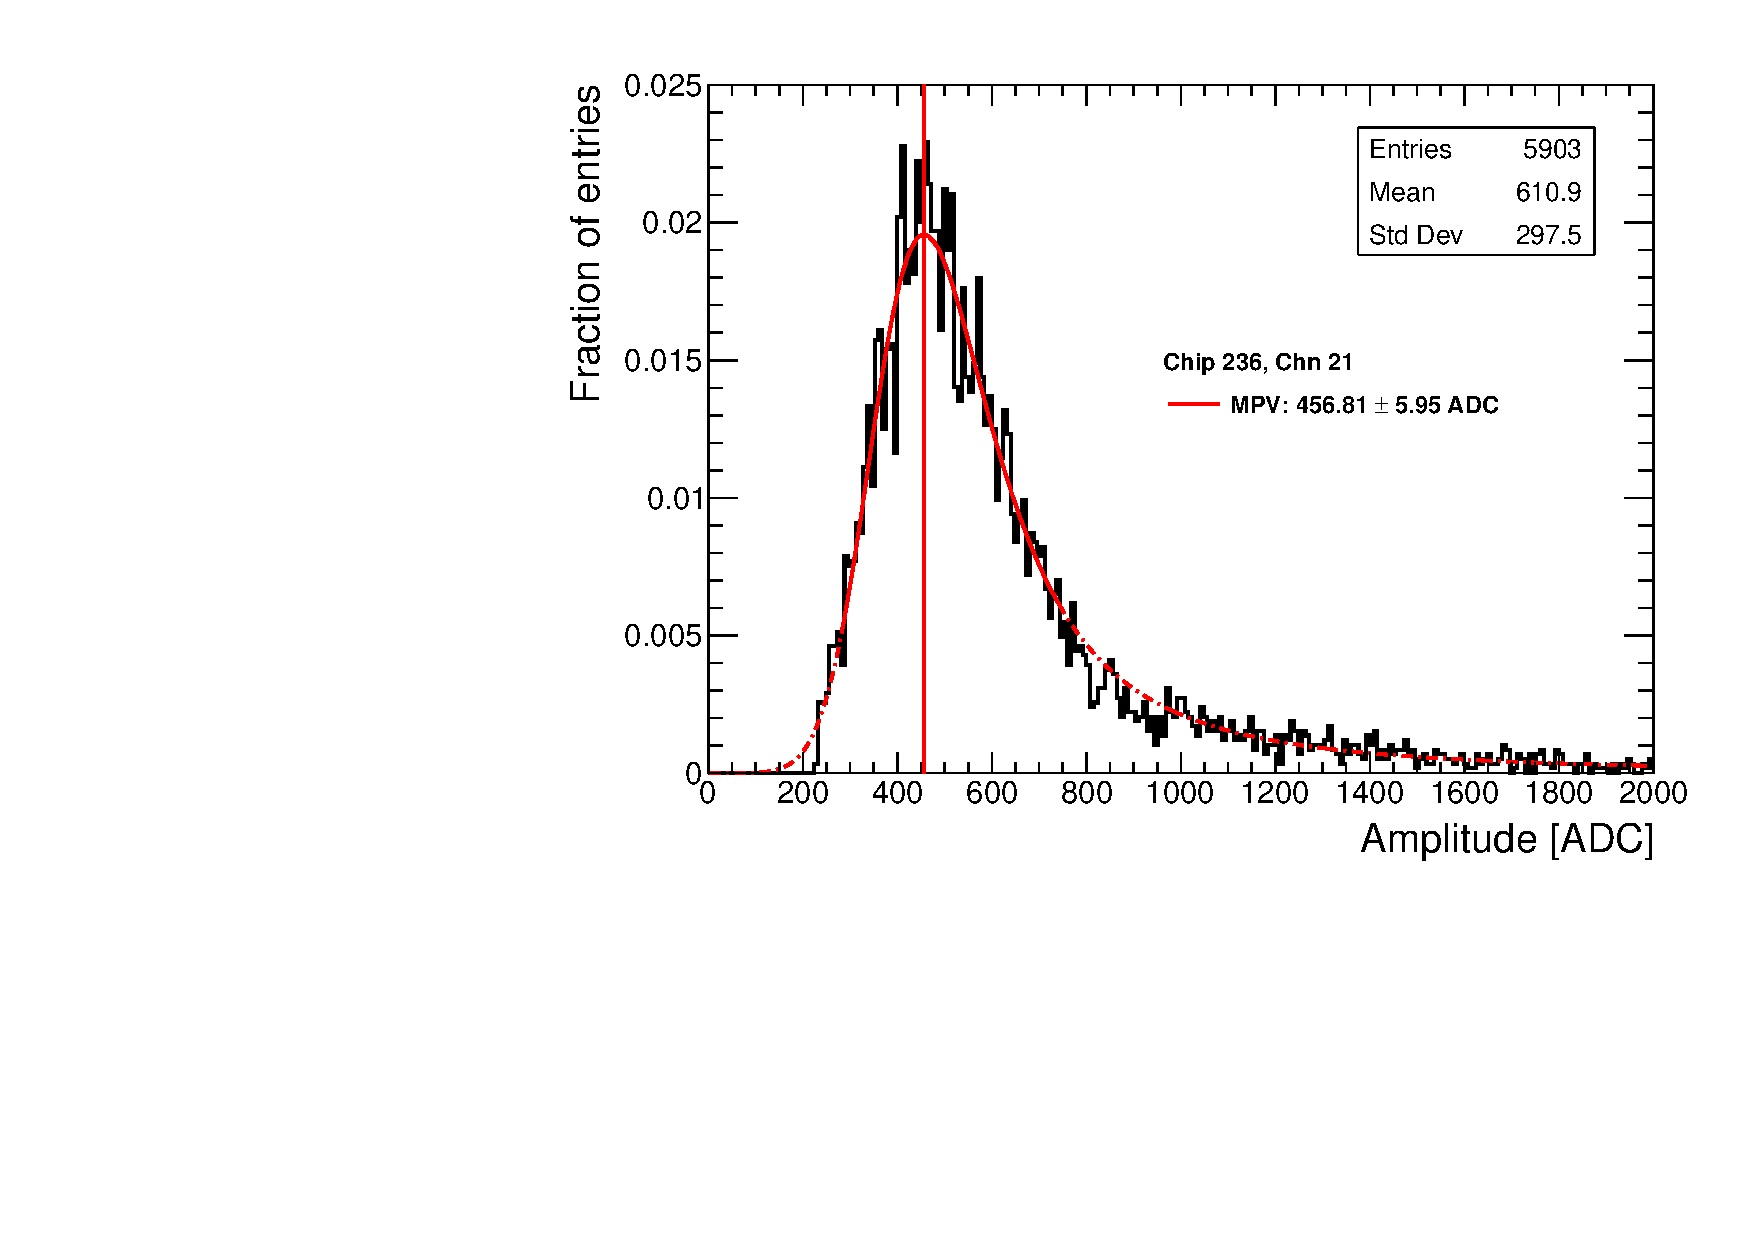
\includegraphics[width=0.7\linewidth]{../Thesis_Plots/EnergyCalib/Plots/ExampleMIP_Module3.pdf}
	\caption{Typical energy distribution in a single channel of the AHCAL.} \label{fig:MIPFit}
\end{figure}

In this way, for the testbeam in July 2015, 72\% of the channels are fitted (over 3744 channels). This does not mean that 28\% of channels are dead (around 15\% of the channels are considered dead), as for the most part, the outer channels of the big layers don't have enough statistic to perform a fit. For centered chips, where channels are not fitted, the mean MPV value of a chip or layer is used. In this way, 83\% of the channels are completed. In order to have a value for each channel, especially for the big layers, the values are combined with previous testbeams performed in April and May 2015 with the big layers. In this way, all 3744 channels have a MIP constant.

\section{Calibration Results}

In this section, a small assessment of the performance of the detector calibration is performed.

\subsection{Error on the calibration}

After the calibration, it is necessary to evaluate the performance of the calibration procedure by looking at the relative error on the extracted MPV value for a MIP. The figure \ref{fig:MIPError} shows the relative error computed for all the channels of the detector. The relative error on the MIP value is for most of the channels in the expected range of 1 to 3\%. Though some higher values can be seen, this comes from the uncalibrated channels that derived their MIP value from the mean of the chip or layer mainly located in the small layers but for the analysis most of them are rejected later on by the list of dead channels due to the lack of gain value or pedestal value.

\begin{figure}[htbp!]
	\centering
	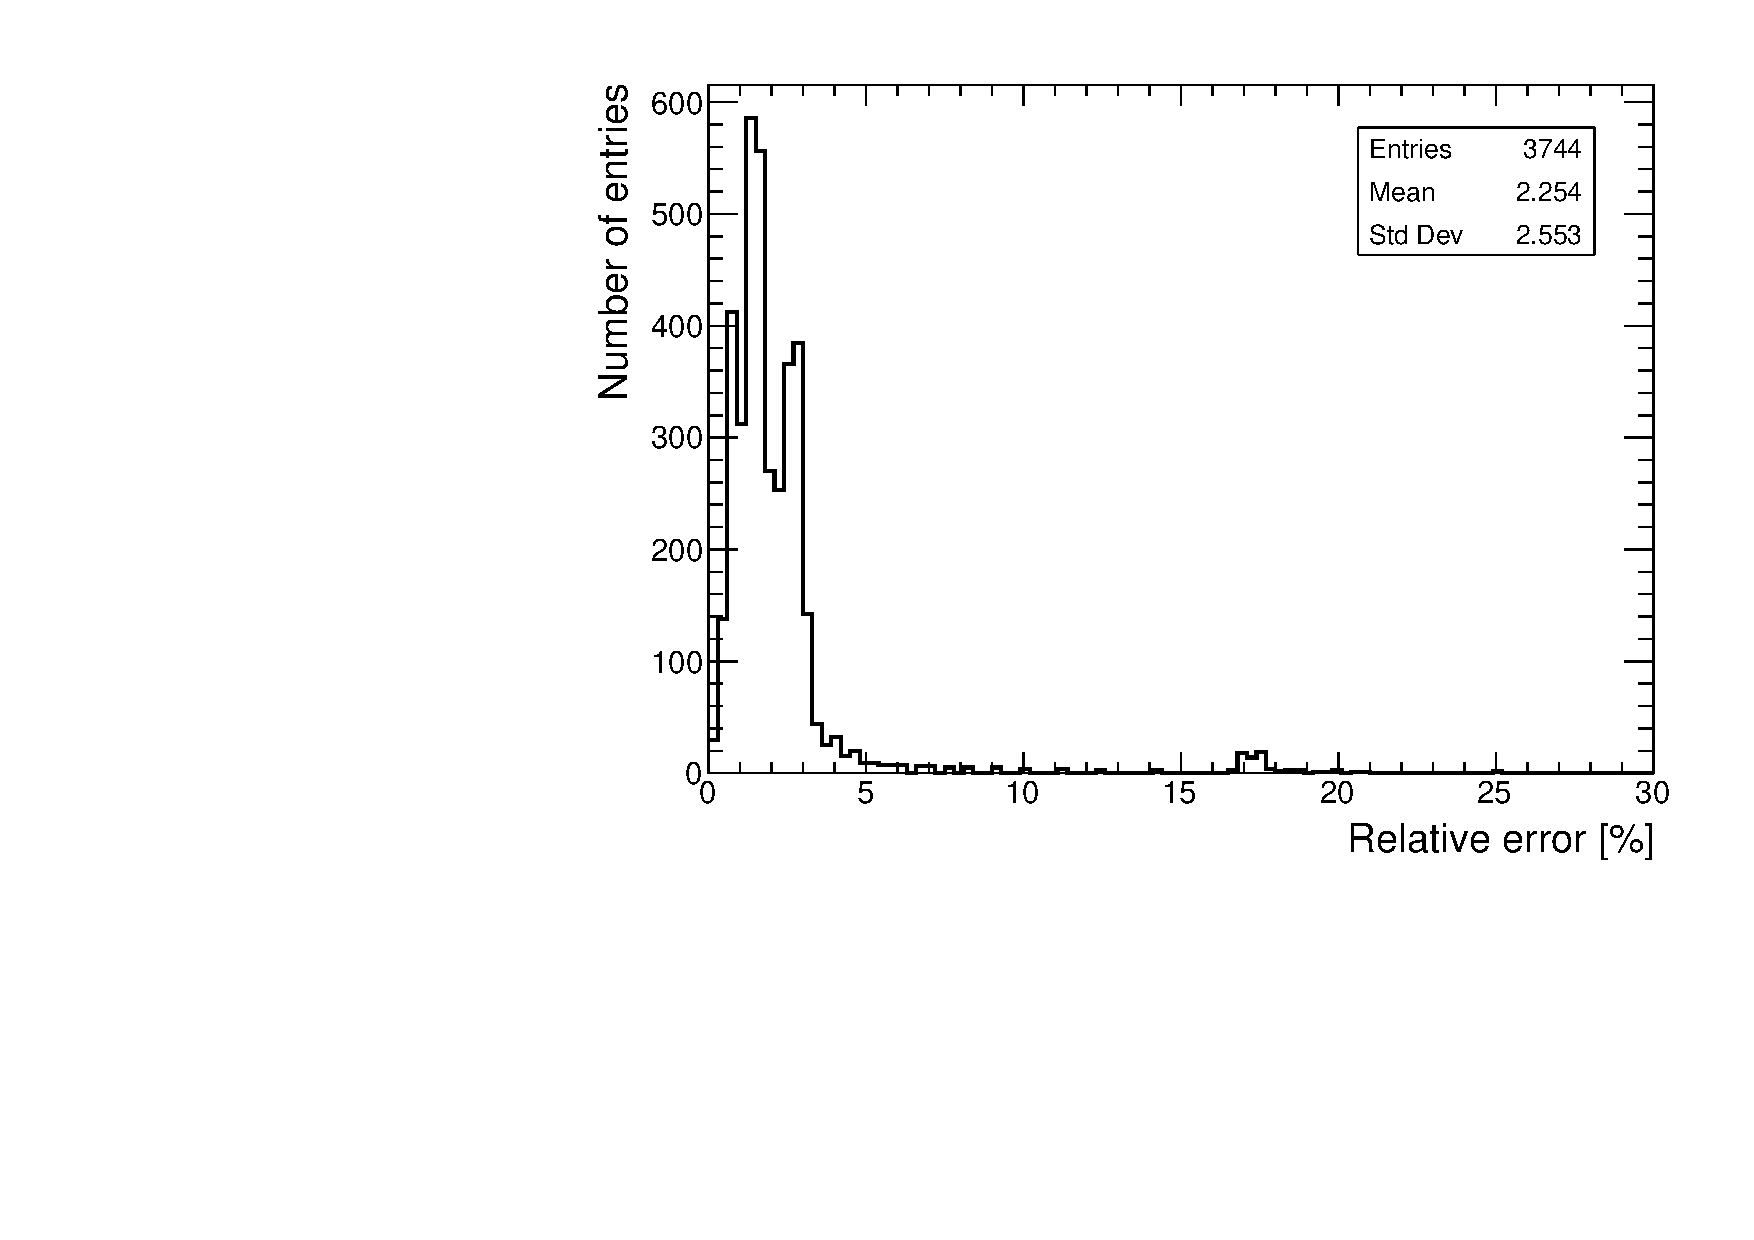
\includegraphics[width=0.7\linewidth]{../Thesis_Plots/EnergyCalib/Plots/RelativeErrorMIP_Combined.pdf}
	\caption{Relative error of the MIP value extracted.} \label{fig:MIPError}
\end{figure}

\subsection{Comparison with simulation}

The MIP calibration defined the energy scale for measure energy depositions in the AHCAL. It is needed to carefully calibrate and validate the MIP calibration in data and simulation in order to get comparable results. Applying the MIP selection, it results into energy depositions of single MIP amplitudes for all channels. The comparison of the MIP spectrum for the whole AHCAL between data and simulation in figure \ref{fig:MIPData_MC} shows that the shape of the hit energy spectrum matches relatively well. The data appears slightly wider than for simulation as channel-wise mis-calibration are not modeled in simulation. This comparison validates the digitization of scintillator-SiPM readout calorimeters.

\begin{figure}[htbp!]
	\begin{subfigure}[t]{0.5\textwidth}
		\centering
		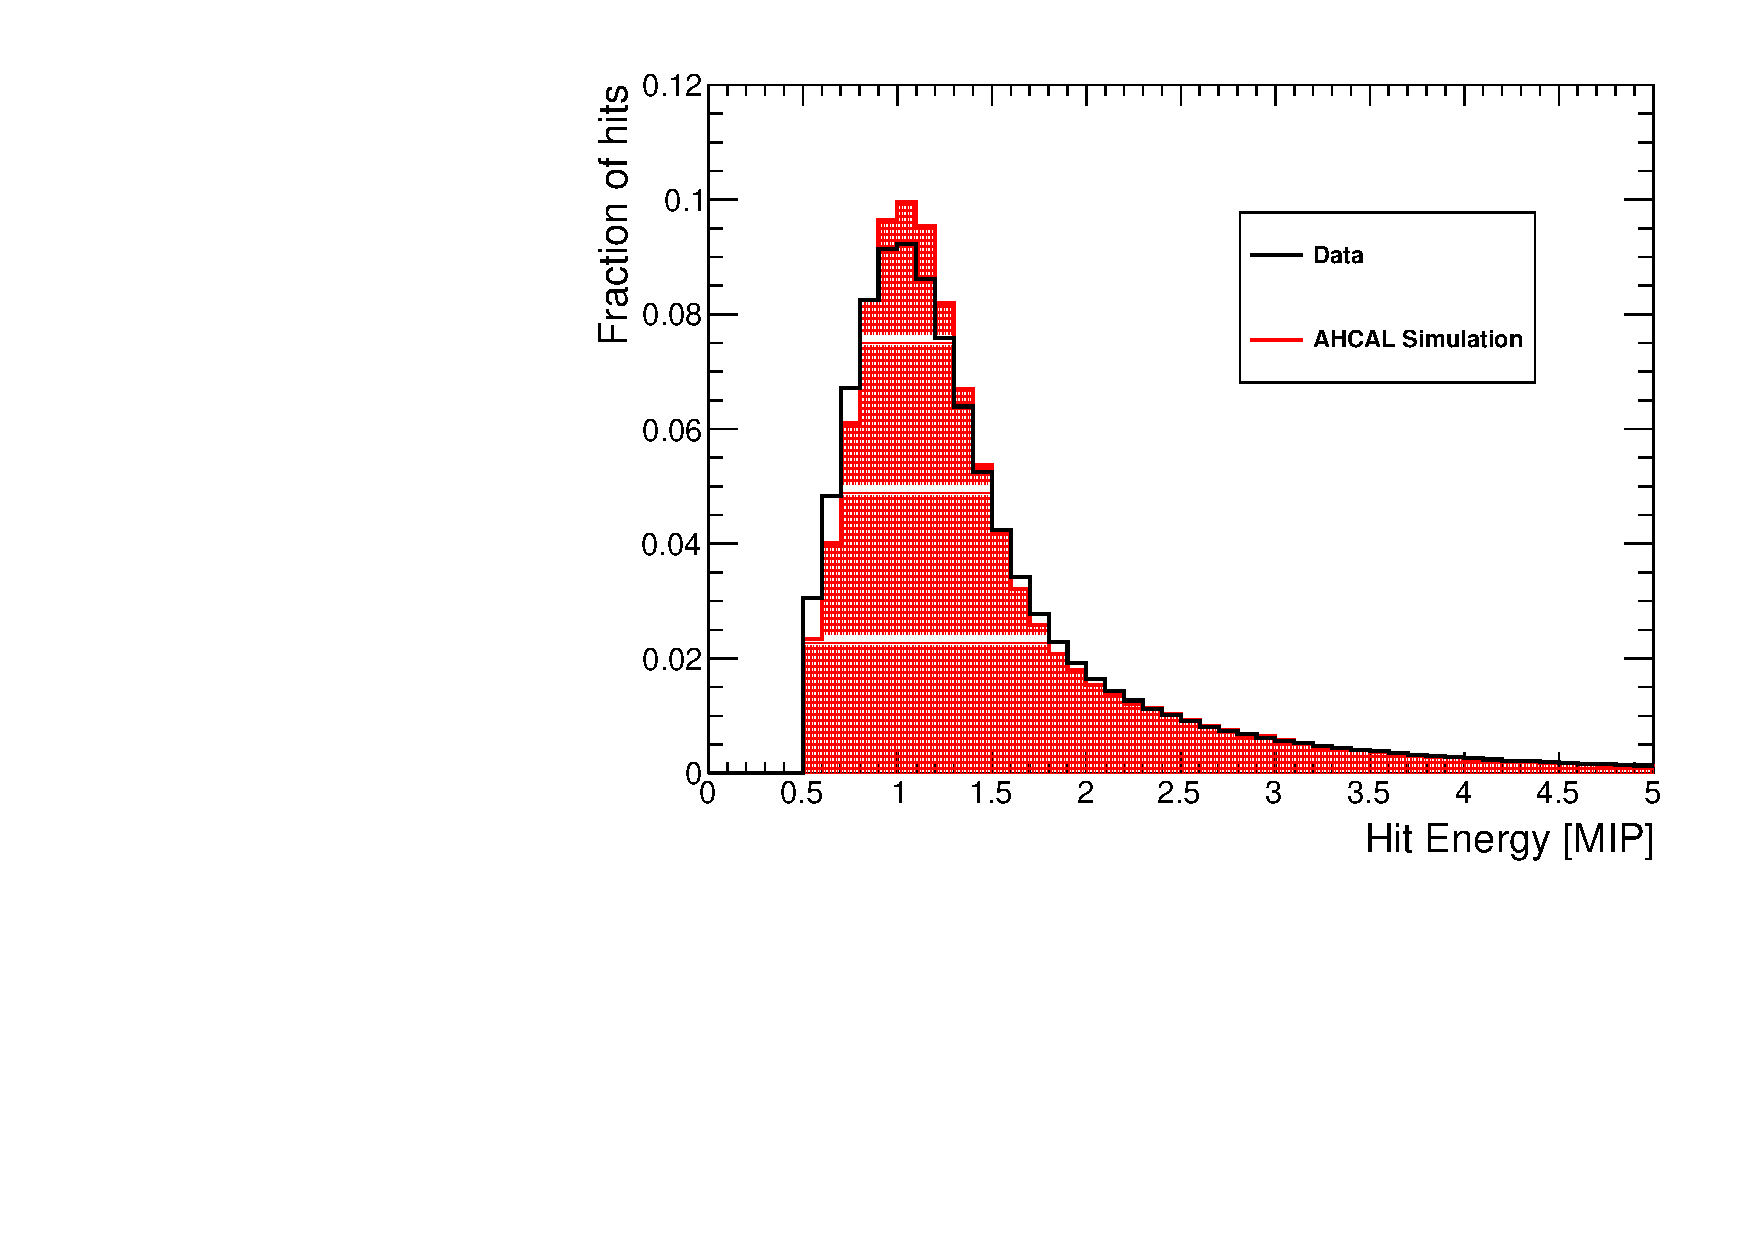
\includegraphics[width=1\linewidth]{../Thesis_Plots/EnergyCalib/Plots/ComparisonMCData_MIPPeak.pdf}
		\caption{} \label{fig:MIPData_MC}
	\end{subfigure}
	\hfill
	\begin{subfigure}[t]{0.5\textwidth}
		\centering
		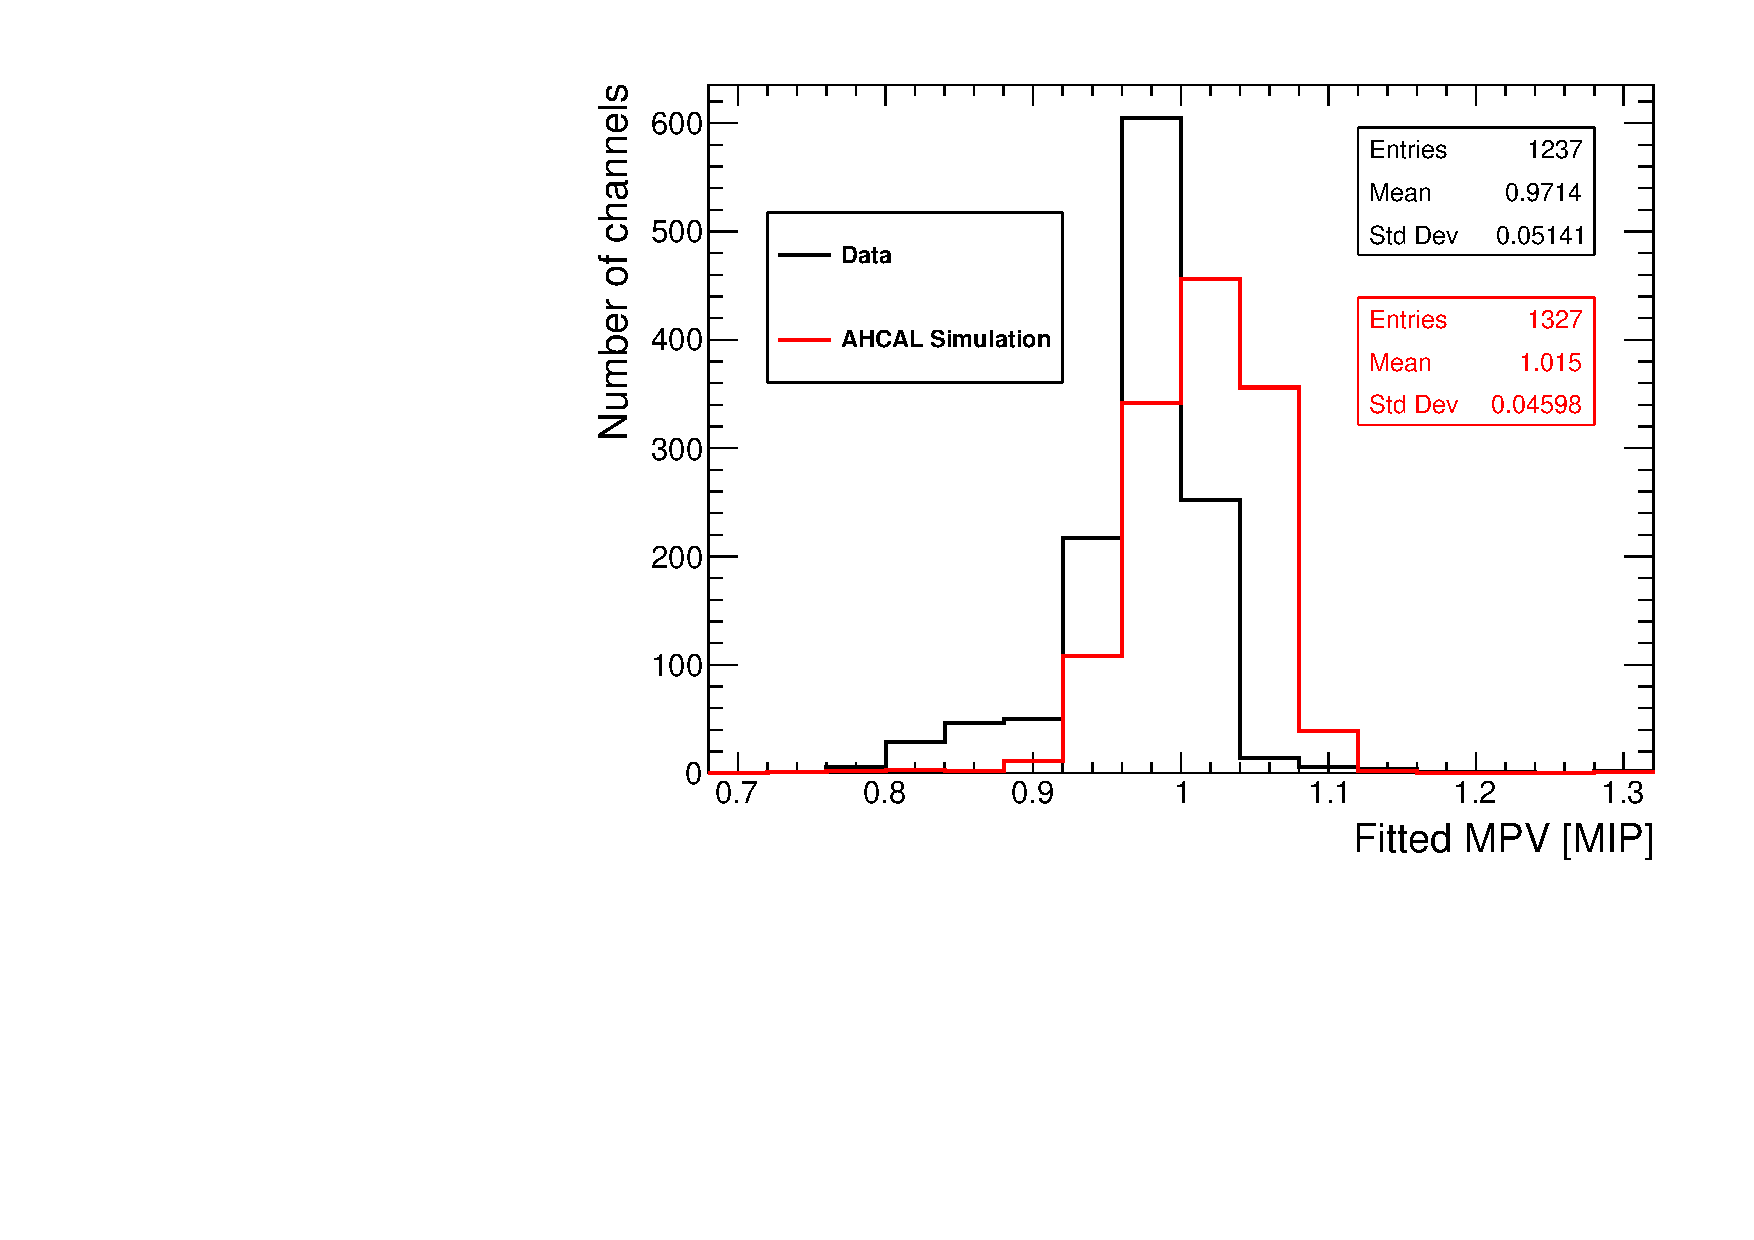
\includegraphics[width=1\linewidth]{../Thesis_Plots/EnergyCalib/Plots/ComparisonMCData_MPV.pdf}
		\caption{} \label{fig:MPVData_MC}
	\end{subfigure}
	\caption{\subref{fig:MIPData_MC}) Hit Energy Spectra for the complete AHCAL for muon like-track hits. \subref{fig:MPVData_MC}) Distribution of fitted MPV in single channels of the AHCAL.}
\end{figure}

The extraction of the MPV value in data and simulation has been done for each single channels of the AHCAL. The figure \ref{fig:MPVData_MC} shows the obtained distribution. Ideally, the fitted MPV should be at 1 for all chips. But in practice, due to mis-calibrations and statistics limitation this results in a widening of the distribution. Both data and simulation give a mean value around 1 MIP for the AHCAL indicating a good average calibration at the cell level. The AHCAL data is slightly shifted to the left to lower values but still reasonably close to unity.

\subsection{Systematic on the MIP scale}

A systematic error on the MIP scale can be derived by divided the muon sample into two sub-samples by even or odd run number. This is will take into account not only the error on the MIP calibration but as well variations due to temperature or temporal variations. Then each samples are fitted using the same fitting procedure as described above.

\begin{figure}[htbp!]
	\centering
	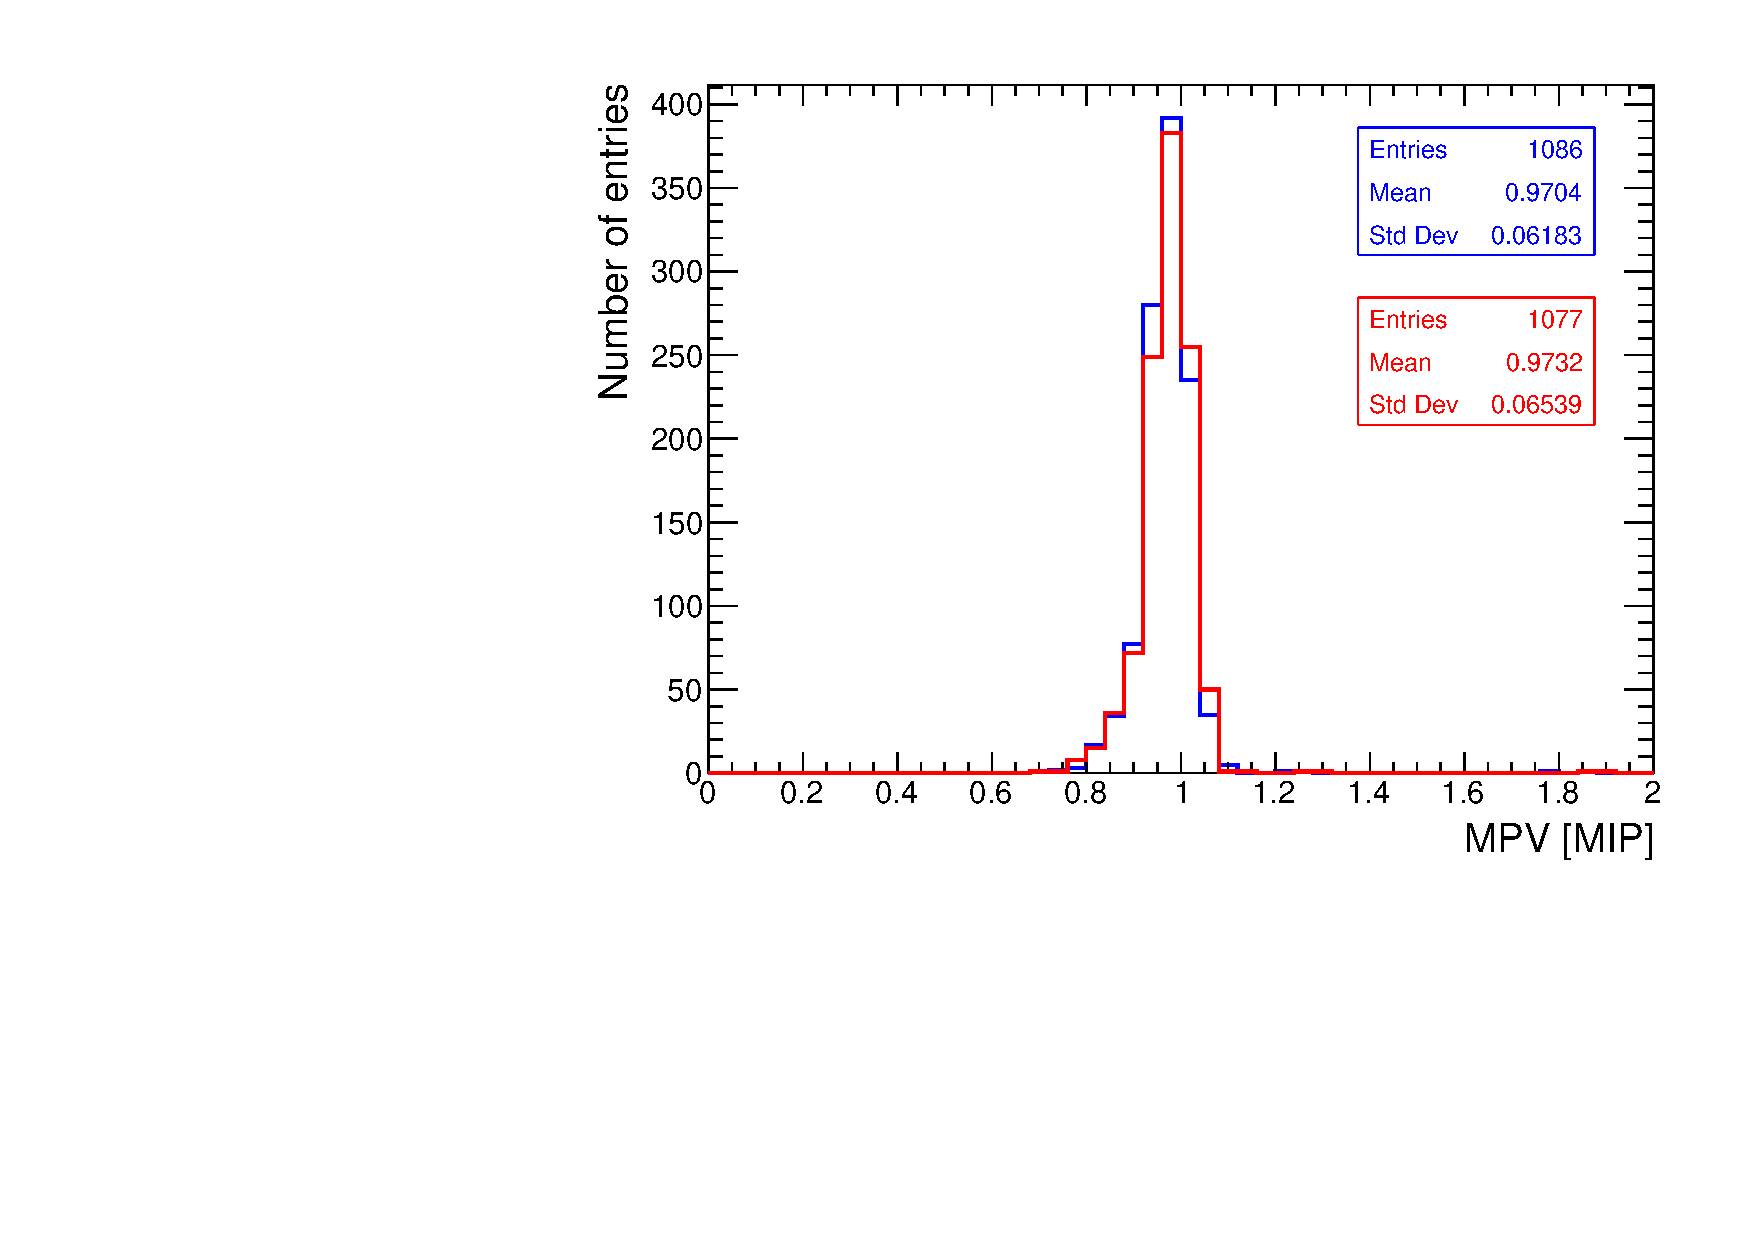
\includegraphics[width=0.7\linewidth]{../Thesis_Plots/EnergyCalib/Plots/SystematicMIP.pdf}
	\caption{MPV fitted value in MIP for the two muon sub-samples. Even runs are in blue, odd runs are in red.} \label{fig:MIPSyst}
\end{figure}

One can see that both samples are very similar with less than 1\% shift in the mean value. By taking the average of the RMS of the distributions, a systematic uncertainty of 6\% on the MIP scale can be derived. This systematic can be used later \ref{} when comparing the mean time of first hit versus the hit energy deposition.

\section{Conclusion}

This chapter presents the results of the MIP calibration obtained for the AHCAL technological prototype installed in the CERN SPS testbeam area in July 2015. The MIP calibration procedure was explained and developed in order to accommodate for such high number of channels as well as the diversity in SiPM types and tile designs. In this way, 83\% of the channels in the detector have their MIP constant determined. An error around 2\% is made on the MIP constant value which is in the order of magnitude expected due to the limited statistics. In order to validate the calibration and the simulation, comparisons have been made at the single channel level. Both data and simulation are in a good agreement though simulation is narrower due to mis-calibration channel-wise not being modeled. A systematic error of around 6\% had been determined on the MIP scale due to run and environmental variations.
